\documentclass[a4paper]{article}

\newif\ifdraft
\drafttrue
%\draftfalse

\usepackage{graphicx}
\usepackage{twocolpceurws}
\usepackage{xspace}
\usepackage{color}
\usepackage[usenames,dvipsnames]{xcolor}

\ifdraft
  \newcommand{\grex}[1]{{\color{red}\emph{Gregorio says: #1}}\xspace}
    \newcommand{\rnombela}[1]{{\color{blue}\emph{Roberto says: #1}}\xspace}
  \newcommand{\cn}{\textcolor{pink}{[citation needed]}}
\else
  \usepackage[disable]{todonotes}
  \newcommand{\grex}[1]{}
  \newcommand{\rnombela}[1]{}
  \newcommand{\fixme}[1]{}
  \newcommand{\cn}{}
\fi

\let\labelindent\relax
\usepackage[inline]{enumitem}

\newcommand{\RQ}[1]{\emph{RQ\textsubscript{#1}}}
\newcommand{\HP}[1]{\emph{H\textsubscript{#1}}}
%\newlist{rquestion}{enumerate}{2}
%\setlist[rquestion,1]{label=\RQ{\arabic*.}, itemsep=0cm, topsep=0.1cm, leftmargin=3.4em}
%\setlist[rquestion,2]{label*=\emph{\textsubscript{\arabic*.}}, itemsep=0cm, topsep=0cm, leftmargin=2.6em}

\newcommand{\tbd}{\emph{To be done.}}

\newenvironment{hassanbox}%
{\begin{center}\vspace{1mm}\noindent\begin{Sbox}\begin{minipage}{0.95\columnwidth}}%
{\end{minipage}\end{Sbox}\fbox{\TheSbox}\end{center}\vspace{1mm}}

%%% Local Variables:
%%% mode: latex
%%% TeX-master: "fairness"
%%% End:


\title{An analysis of App Inventor projects}

\author{
Roberto Nombela \\ Universidad Rey Juan Carlos\\
                Madrid, Spain \\ r.nombelaa@alumnos.urjc.es
}

\institution{}

\begin{document}
\maketitle

\begin{abstract}
Visual programming languages help learners to acquire and improve programming and computational skills.
There are many visual programming languages and platforms currently, being Scratch the most popular one.
After Scratch, learners usually move to other visual languages, as for instance MIT App Inventor, a visual programming language block-based to create Android applications.
Many studies exist on the acquisition and assessment of computational thinking skills in Scratch.
However, despite its wide use, similar studies on the use of App Inventor can be seldom found.
That is why in this paper we gather and analyze App Inventor projects with the goal of having an overview of the type of projects that are created.
Our aim in the long run is to create tools that support the learning process of App Inventor.
\end{abstract}


\section{Introduction}

In recent years, the concept of Computational Thinking (CT) has been presented as a process to solve problems, not necessarily only in programming~\cite{wing2006computational}. 
CT includes skills that facilitate the resolution of problems, such as: abstraction, algorithmic and parallel thinking, data representation. These abilities make the CT a fundamental help for any learner.

One way to acquire and improve the skills of CT and programming level are visual programming languages.
This is because programming involves activities such as the ability to design, create and invent new media~\cite{resnick2009scratch}.
The Scratch and App Inventor visual programming languages are examples of this.

Because of this, tools that assess the CT skills from the projects of these programming languages have also emerge, for example Dr. Scratch~\cite{moreno2015dr} and Code Master that analyze the Scratch and App Inventor (and Snap!) projects respectively. 
At current time, these assessmentshave turned out to be more useful for educators than for learners by the fact that the latter do not receive enough feedback to improve (\cn).

\rnombela{This cite is about CTE 2018 paper, can it be cited despite being unpublished?}

This study aims to find a way to help learners improve by analyzing the blocks of App Inventor projects. Observing values as number or variety of blocks we will have an overview of the type of projects that the App Inventor community are creating.

For the analysis, more than 1000 projects obtained from the Gallery of App Inventor web have been used. 
In this Gallery you can find tens of thousands of projects uploaded by users. The age, gender, nationality or level of programming of the users are unknown.

This paper is structured as follows: the Methodology section talks about the acquisition and preparation of the data for the analysis and the Results section shows what has been obtained using the cleaned data. Finally in the Conclusions section we interpret the results.

\section{Methodology}


\subsection{Data Gathering}

The process of data gathering consists of downloading projects from the App Inventor Gallery. In addition to the most popular projects, the most recent ones have also been downloaded, since many projects are being uploaded every day. One problem with this is that you can find many empty (0 blocks) or duplicate projects. Another problem is the difficulty to automate the download process because you have to make a copy of the Gallery projects to your account projects and then download them.

\rnombela{Do I upload the projects to the repo in a zip and share the link?}

Every project has two different types of files per screen, bky and scm. In bky files we can see, in XML format, all the blocks used. While scm files use JSON structure and represent all the components used. Thus, to extract the blocks we run a script that creates a dictionary where the key is the type and the value is the number of blocks of that type, looks at the next block and if it is a new type it is included to the dictionary with value one, otherwise it is added one to the value. Using this script for each project we have all the blocks extracted and classified, so this information is saved in a csv file. Once we have all projects prepared, we must discard empty or duplicate projects.

\rnombela{Do you mean the rubric of Dr. App Inventor?}


\begin{table}[ht]
\begin{center}
\caption{Comparative table of the number of blocks}

\bigskip

\begin{tabular}{|l|l|l|l|}
\hline
& Original & No empty & No duplicate \\ \hline
Frequency & 1222 & 1102 & 730\\ \hline
Mean & 187.89 & 208.35 & 211.48\\ \hline
Std. Dev & 463.68 & 483.9 & 502.62 \\ \hline
Minimum & 0 & 1 & 1\\ \hline
Maximum & 5476 & 5476 & 5476 \\ \hline
\end{tabular}
\end{center}
\end{table}

Next, the ``used blocks'' are studied, that is, each type of block adds one for each project in which it has been used. The ``repeated blocks'' are also studied: we add the number of each type of blocks used in each project. We can see that the correlation of both is 0.84, which means that they are highly related.

\section{Results}

Counting the most and least used blocks for all projects we obtain:

\begin{table}[ht]
\begin{center}
\caption{Most used blocks}

\bigskip

\begin{tabular}{|l|l|}
\hline
component\_set\_get & 28927\\ \hline
text & 22644\\ \hline
math\_number & 15308\\ \hline
lexical\_variable\_get & 14662\\ \hline
component\_event & 9599\\ \hline
\end{tabular}
\end{center}
\end{table}

\begin{table}[ht]
\begin{center}
\caption{Least used blocks}

\bigskip

\begin{tabular}{|l|l|}
\hline
controls\_closeScreenWithPlainText & 1\\ \hline
math\_tan & 2\\ \hline
obfuscated\_text & 2\\ \hline
text\_is\_string & 2\\ \hline
list\_to\_csv\_table & 3\\ \hline
\end{tabular}
\end{center}
\end{table}

While for projects with a variety less than 10:

\begin{table}[ht]
\begin{center}
\caption{Most used blocks for small projects}

\bigskip

\begin{tabular}{|l|l|}
\hline
component\_set\_get & 5562\\ \hline
text & 4538\\ \hline
component\_event & 3960\\ \hline
component\_method & 3484\\ \hline
controls\_openAnotherScreen & 1277\\ \hline
\end{tabular}
\end{center}
\end{table}

\begin{table}[ht]
\begin{center}
\caption{Least used blocks for small projects}

\bigskip

\begin{tabular}{|l|l|}
\hline
text\_trim & 0\\ \hline
math\_divide & 0\\ \hline
math\_cos & 0\\ \hline
controls\_forEach & 0\\ \hline
math\_convert\_number & 0\\ \hline
\end{tabular}
\end{center}
\end{table}


\subsection{Study of the scores depending on the variety.}

The distribution of the variety of blocks (number of different blocks used) for each project can be seen in the following figure:

\begin{figure}[ht]
\begin{center}
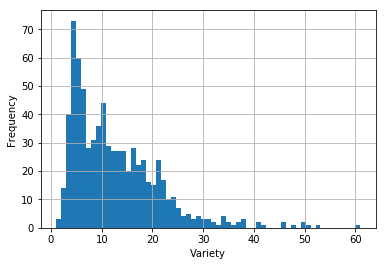
\includegraphics[height=4cm]{fig1}
\caption{Variety distribution }
\label{fig1}
\end{center}
\end{figure}

Projects with more than 10 blocks represent 48.2\% (352 of 730) of the blocks and the scores can be characterized as seen in the following table versus the scores of the projects with less than 10 blocks:

\begin{table}[ht]
\begin{center}
\caption{Comparative table of scores between small and large projects}

\bigskip

\begin{tabular}{|l|l|r|}
\hline
& Large projects & Small projects \\ \hline
Frequency & 352 & 378\\ \hline
Percentage & 48.2 & 51.8\\ \hline
Mean & 18.56 & 9.89\\ \hline
Std. Deviation & 5.33 & 3.27\\ \hline
Minimum & 7 & 3\\ \hline
Maximum & 36 & 19\\ \hline
\end{tabular}
\end{center}
\end{table}


\subsubsection{Acknowledgements}

eMadrid. TBD


\bibliographystyle{alpha} 
\bibliography{samplebib}
%inline the .bbl file directly for mailing to authors.

\end{document}


